\documentclass[conference]{IEEEtran}
\usepackage{graphicx}
\usepackage[cmex10]{amsmath}
\usepackage{enumitem}
\usepackage{tikz}
\usetikzlibrary{calc}
\usepackage[backend=biber,style=ieee,bibstyle=authortitle,sorting=none]{biblatex}
\addbibresource{lib.bib}

\begin{document}

\title{Creating data associations over different file types without supervision}
\author{\IEEEauthorblockN{Marcus Schlutter}
\IEEEauthorblockA{Siemens AG\\
		  Chemnitz, Germany\\
		  marcus.schlutter@etit.tu-chemnitz.de}
}

\maketitle

\begin{abstract}
This document proposes an unsupervised learning algorithm to match file content / data
associations in different file types for the purpose to use the associations to generate
one file from the other. The proposal is independent from the underlying data but
dependents on the arrangment of the data which must support a path-like addressing scheme
to select the correct path based on simple majority.
\end{abstract}

\begin{IEEEkeywords}
Unsupervised learning, machine learning, file generation, data associations, Office
digitalization, XML
\end{IEEEkeywords}

\section{Introduction}
The presence of programs like \textit{Datatap} \cite{adverity:adverity} or \textit{MapForce}
\cite{altova:mapforce} show that there's a demand for programs which are capable of extracting
data from one file (format) to another. Both solutions however lack the automization in the
meaning that manual interaction is required to create associations. Here an approach is proposed
to overcome this limitation by automatically create associations without the application of
neuronal networks in favor of traceability.\\
The proposal is first explained in an abstract manner in the \textit{Procedure}-section and
will later shown on an example which should give the reader a better grasp of an
implementation.

\section{Requirements}
For the proposed algorithm to work as expected some prerequisite have to be formulated:
\begin{enumerate}[label=(\roman*)]
% \item The data to be associated represents complex data structures which occur multiple
%        times ie. it is a list of objects
 \item Files should be separable into 2 groups: one being the \textit{target}-group containing
        only one file \footnote{technically multiple files should be possible but this is
        discouraged}. While the other group is the \textit{source}-group
 \item Both groups contain the same data represented in complex structures which occur multiple
        times ie. it is a list of objects. For the \textit{source}-group this data pool can be
        only a subset of the data contained.
 \item In both groups the contained data is arranged in a way that every field of this complex
        data structures can be addressed individually.
 \item The data within this data structures need to be heterogenous (between the different
        fields) with a significant number of data structures / objects.
\end{enumerate}

\section{Procedure}
The algorithm can be separated in 3 functional steps: the collection-phase, the selection-phase
and the generation (of the \textit{target}-file).\\All steps build one a central internal data
structure which can be visualized as a 2-dimensional histogram which stores path-pairs as their
occurances.

\subsection{Collection-Phase}
All values available in the first file ie. \textit{target}-file are to be extracted and
paired with their addressing path. Paths should be constructed independent of the current
complex structure but specific to they field they represent. In the next step this
collection is compared against the values in the group of \textit{source}-file(s) were
every match is recorded in the forementioned 2-dimensional histogram. Figure
\ref{classifier_table} shows an examplary arrangment. In the next step the collected data
is evaluated.
\begin{figure}[h]
  \centering
  \scalebox{0.64}{
  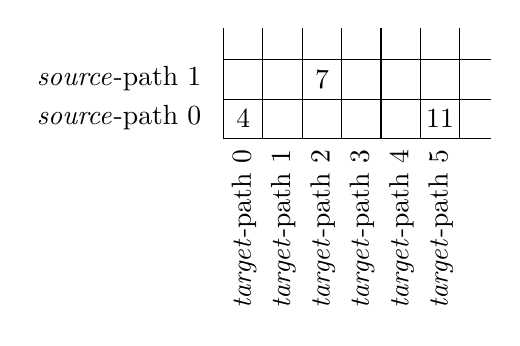
\begin{tikzpicture}
   \draw (1,2.4) -- (1,1) -- (4.4,1);
   \draw[step=0.5] (1,1) grid (4.4,2.4);
   \foreach \x/\i in {1.1/0, 1.6/1, 2.1/2, 2.6/3, 3.1/4, 3.6/5}
    \node[label={[label distance=-6.5em, text depth=-1ex,rotate=90]right: \textit{target}-path \i}]
          at (\x,1) {};
   \foreach \y/\i in {1.3/0, 1.8/1}
    \node[label={[label distance=1, text depth=-1ex]left: \textit{source}-path \i}]
            at (1,\y) {};
   \node at (1.25,1.25) {4};
   \node at (2.25,1.75) {7};
   \node at (3.75,1.25) {11};
 \end{tikzpicture}}
 \caption{2-dimensional histogram for storing path-pairs}
 \label{classifier_table}
\end{figure}

\subsection{Selection-Phase}
In this step from all possible path combinations the one considered correct is to be selected.
This is resolved interpreting the problem as a simple case of the \textit{Byzantine Generals
Problem} as described in \cite{lamport:byzantine}. From this concept also the limitations can
be inherited: for every path-match $p_i$ the final pair $p$ is derived via
$majority(p_1, p_2, ...,p_n)$ under the assumption that $n \geq 2k + 1$ with $k$ being the
count of errors. An error might manifest either as a wrong path-pair due to the value is
matched multiple times for different data structure fields or a correct match could not be
made due to the \textit{target}-file containing a false value (compared to the content of
the corresponding \textit{source}-file). Which introduces a certain robustness against
human errors unintentionally inserted when creating former target files.

\subsection{Generation}
After all matches had been made correctly (intervention is possible by manually altering the
histogram-structure) the \textit{target}-file can be derived from the \textit{source}-files in
case the later are modified or extended. Structural changes can be compensated by ``re-training''
the system.\\As the main goal of the algorithm is to pick the right ``bin'' in the histogram it
has been named \textit{Naive PathClassifier}.

\section{Implementation example}
To give the reader a better idea of the application and the limits of the algorithm this section
will give an in-depth view in the prototype which was created as a demonstrator. As mocking
data a XML- and multiple docx-file(s) about a fictitious company was created. The XML-file (as
the file to generate) contained data that could be completly found in the docx-files: this was
data to describe the departments and the workers of that company. The departments were described
with properties like:\newline
name of the department, the workers associated, teams in the department with a name and a worker
count.\newline
Workers had properties like:
an ID, a name, profession, etc.\newline
In the XML-file worker-trees (ie. data structures) and department-trees were child nodes to
respective nodes creating 2 separate lists in the XML within a greater tree. Data in the
docx-files was organized in tables with one main docx-files and references to other
docx-file in the main file. The worker to  department association was expressed as a table
like shown in figure \ref{cross_table}. All table headers had a distinctive background color.
\begin{figure}[h]
 \centering
 \scalebox{0.64}{
 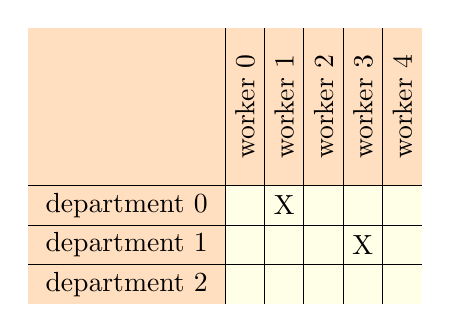
\begin{tikzpicture}
  %\draw(1.5,0) -- (1.5,1.5) -- (4,1.5);
  \fill [orange!25] (-1,0) rectangle (4,3.5);
  \fill [yellow!10] (1.5,0) rectangle (4,1.5);
  \foreach \x in {1.5,2,2.5,3,3.5}
    \draw (\x,0) -- (\x,3.5);
  \foreach \x/\i in {1.75/0,2.25/1,2.75/2,3.25/3,3.75/4}
    \node[rotate=90] at (\x,2.5) {worker \i};
  \foreach \y in {0.5,1,1.5}
    \draw (-1,\y) -- (4,\y);
  \foreach \y/\i in {0.25/2,0.75/1,1.25/0}
    \node at (0.25,\y) {department \i};
  \node at (2.25,1.25) {X};
  \node at (3.25,0.75) {X};
 \end{tikzpicture}}
 \caption{Department to worker association as a \textit{cross table}}
 \label{cross_table}
\end{figure}

\subsection{Project organisation}
To extract the paths from the XML and the docx-files for both types wrappers / translators
were created. For the XML-wrapper a subset of XPath could be used as output while for the
docx-files an own scheme had to be created using the file name, the sheet, the column and
row. The project structure explained in this section is displayed in figure
\ref{project_structure}.
\begin{figure}[h]
 \centering
 \includegraphics[scale=0.16]{img/ProjectStructure_en}
 \caption{Project organisation for example project}
 \label{project_structure}
\end{figure}
To yield a more robust matching the XML-wrapper would create triples of
the form: XML-path, object-ID and field-value. The XML-tag for the name of the root-node and
the node of the object-ID were provided via a config-file. Having the ID and the associated
value allowed to detect the orientation of a docx-table which the wrapper knew 3 types of:
a horizontal aligned table, a vertical one and the cross table displayed in figure
\ref{cross_table}. The table header (of different color) was detected to point to the first
field which simplified matching in the classifier and the file generation. Matching with the
name cell ``position'' also increased robustness in case the objects would be unordered in
the tables. As a final step the target-file was stripped of its object entries in the list
nodes and used as template for files to generate.

\subsection{Example results}
Figure \ref{example_table} shows the result for the prototype with the company employing 20
workers. The algorihm broke with a worker count below 11 as the department sizes interfered
with the team sizes within the docx-files (violation of the inhomogenity requirement).
\begin{figure}[ht]
 \centering
 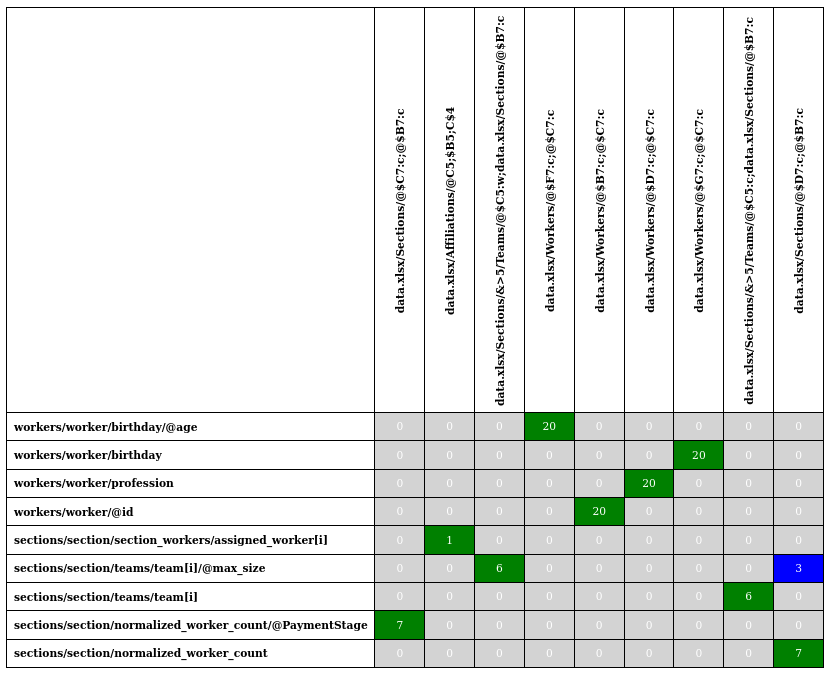
\includegraphics[scale=0.42]{img/example_table}
 \caption{Collection and Selection result for 20 workers distributed over 6 sections}
 \label{example_table}
\end{figure}

\section{Summary}
In this document an algorithm was presented which is capable of ``learning'' data
associations unsupervised  between different file types with matching wrappers present.
The solution was named \textit{Naive PathClassifier}. This algorithm decides over
associations by majority of path-pairings which worked well in a case study presented
as an example. 

\printbibliography

\end{document}
